\section{Wien-Robinson-Brücke}
\label{sec:Wien-Robinson-Brücke}

\subsection{Durchführung}
\label{subsec:Durchführung}

Die Wien-Robinson-Brücke ist die erste der genannten Brücken, die 
Frequenzabhängig ist. Diese Abhängigkeit bedeutet, dass ein Abgleich
der Widerstände nur bei einer bestimmten Frequenz durchgeführt werden 
kann. Diese soll untersucht werden. 

\begin{figure}
    \centering
    \begin{tikzpicture}[circuit ee IEC, font=\sffamily]
    \draw [->] (0,-3.5) -- (0, -2);
    \draw (-0.5,-2) -- (0.5,-2);
    \node[scale=0.8] at (0,-4) {$U_s$};
    \draw [->] (0,-4.5) -- (0, -6);
    \draw (-0.5,-6) -- (0.5,-6);
    \draw (1,0) to [AC source](1,-8);
    \node[contact] at (1,-2) {};
    \node[contact] at (1,-6) {};
    \draw (1,0) -- (4,0);
    \draw (4,0) -- (4,-1);
    \draw (2.5, -1) -- (5.5,-1);
    \draw (2.5, -1) to [resistor={info={$2R'$}}] (2.5, -4);
    \draw (5.5,-1) to [capacitor={info={C$\mathsf{_{}}$},info'={$\mathsf{_{}}$}}] (5.5,-2.5);
    \draw (5.5,-2.5) to [resistor={info={$R$}}] (5.5, -4);
    \node[contact] at (4, -1) {};
    \node[contact] at (2.5,-4) {};
    \node[contact] at (3.5,-4) {};
    \node[contact] at (4.5,-4) {};
    \node[contact] at (5.5,-4) {};
    \draw (2.5, -4) -- (3.5, -4);
    \draw (4.5, -4) -- (5.5, -4);
    \draw (2.5,-4) to [resistor={info={$R'$}}] (2.5, -7);
    \draw (2.5, -7) -- (5.5, -7);
    \draw (5.5,-4) to [capacitor={info={C$\mathsf{_{}}$},info'={$\mathsf{_{}}$}}] (5.5,-7);
    \node[contact] at (5.5, -7){};
    \draw (5.5, -4) -- (6.5, -4);
    \draw (5.5, -7) -- (6.5, -7);
    \draw (6.5, -4) to [resistor={info={$R$}}] (6.5, -7);
    \draw (4, -7) -- (4, -8);
    \draw (1,-8) -- (4, -8);
    \node[contact] at (4, -7);
    \node[scale=0.8] at (4,-4) {$U_b$};
    \end{tikzpicture}
    \caption{Induktivitätsmessbrücke}
    \label{fig:Induktivitätsmessbrücke}
\end{figure}

Die Frequenz $f$ der Speisespannung $U_s$, die im Bereich 20-30 kHz liegt, 
wird dabei in um die Minimalbrückenspannung kleiner werdenden Abständen variiert. 
Aufgezeichnet wird dabei die Brückenspannung $U_b$. Zum Schluss wird die auch 
die Speisespannung $U_s$ aufgezeichnet. 
 
\subsection{Auswertung}
\label{subsec:Auswertung}

\begin{figure}
  \centering
  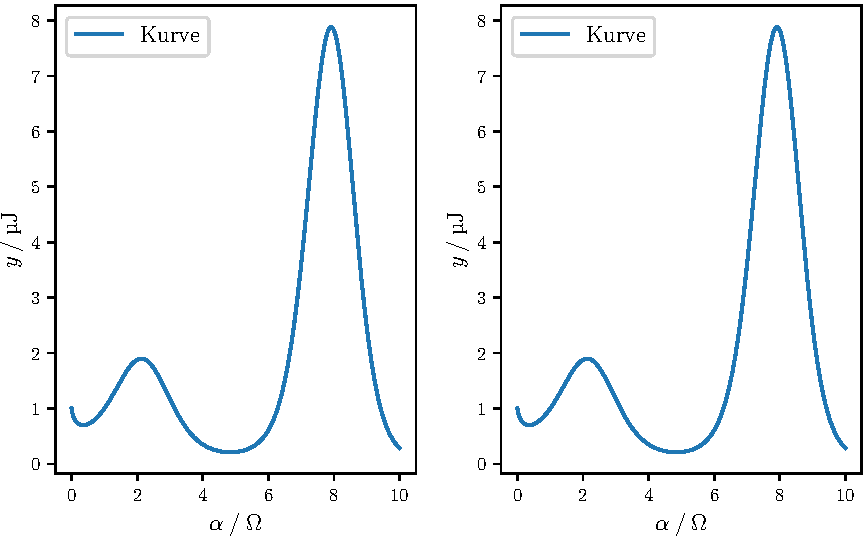
\includegraphics{plot.pdf}
  \caption{Plot.}
  \label{fig:plot}
\end{figure}